\documentclass[tikz,border=2pt]{standalone}
\usepackage[T1]{fontenc}
\usepackage{lmodern}
\usepackage{amsmath}
\usepackage[table]{xcolor}
\usepackage{tikz}
\usetikzlibrary{arrows.meta,calc,positioning}

\definecolor{paletteGreen}{HTML}{2A6F62}
\definecolor{paletteOrange}{HTML}{D96C3D}
\definecolor{darkblue}{RGB}{30,60,120}
\definecolor{fedbuffteal}{HTML}{1D7A73}
\definecolor{fedstalebrown}{HTML}{8A5A2B}

\begin{document}
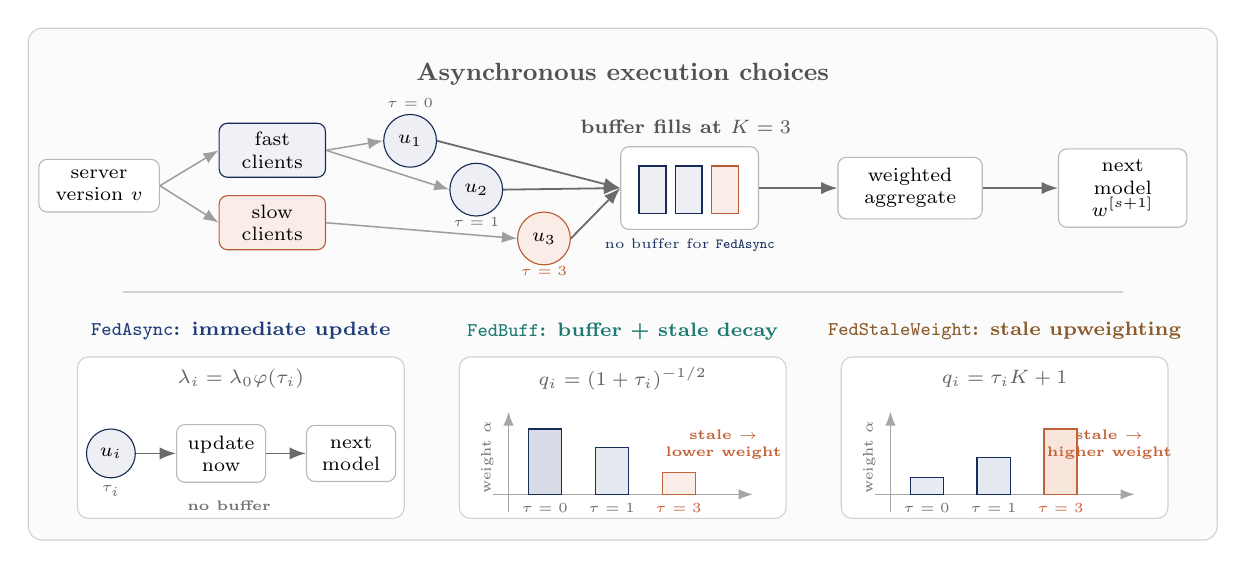
\begin{tikzpicture}[
  >=Latex,
  font=\scriptsize,
  outer/.style={draw=black!18, fill=gray!3, rounded corners=5pt, minimum width=15.1cm, minimum height=6.5cm},
  panel/.style={draw=black!18, fill=white, rounded corners=4pt, minimum width=4.15cm, minimum height=2.05cm},
  clientfast/.style={draw=darkblue!70!black, fill=darkblue!7, rounded corners=3pt, align=center, minimum width=1.35cm, minimum height=0.55cm},
  clientslow/.style={draw=paletteOrange!85!black, fill=paletteOrange!12, rounded corners=3pt, align=center, minimum width=1.35cm, minimum height=0.55cm},
  updatefast/.style={draw=darkblue!70!black, fill=darkblue!8, circle, minimum size=6.7mm, inner sep=0pt, font=\scriptsize\bfseries},
  updateslow/.style={draw=paletteOrange!85!black, fill=paletteOrange!13, circle, minimum size=6.7mm, inner sep=0pt, font=\scriptsize\bfseries},
  box/.style={draw=black!28, fill=white, rounded corners=3pt, align=center, inner sep=4pt},
  arrow/.style={->, line width=0.65pt, draw=black!58},
  mutedarrow/.style={->, line width=0.55pt, draw=black!38},
  methodarrow/.style={->, line width=0.8pt},
  note/.style={align=center, text=black!62},
  barlabel/.style={font=\tiny, text=black!58, align=center}
]
\node[outer] at (0,0) {};
\node[font=\bfseries\small, text=black!68] at (0,2.67) {Asynchronous execution choices};

\node[box, text width=1.25cm] (server) at (-6.65,1.25) {server\\version \(v\)};
\node[clientfast] (fast) at (-4.45,1.70) {fast\\clients};
\node[clientslow] (slow) at (-4.45,0.78) {slow\\clients};
\draw[mutedarrow] (server.east) -- (fast.west);
\draw[mutedarrow] (server.east) -- (slow.west);
\node[box, minimum width=1.75cm, minimum height=1.05cm] (buffer) at (0.85,1.22) {};
\node[updatefast] (uone) at (-2.70,1.82) {\(u_1\)};
\node[updatefast] (utwo) at (-1.86,1.20) {\(u_2\)};
\node[updateslow] (uthree) at (-1.00,0.58) {\(u_3\)};
\node[barlabel] at (-2.70,2.3) {\(\tau=0\)};
\node[barlabel] at (-1.86,0.79) {\(\tau=1\)};
\node[barlabel, text=paletteOrange!90!black] at (-1.00,0.16) {\(\tau=3\)};
\draw[mutedarrow] (fast.east) -- (uone.west);
\draw[mutedarrow] (fast.east) -- (utwo.west);
\draw[mutedarrow] (slow.east) -- (uthree.west);

\node[font=\scriptsize\bfseries, text=black!68] at (0.8,2) {buffer fills at \(K=3\)};
\draw[draw=darkblue!70!black, fill=darkblue!8, line width=0.55pt] (0.21,0.9) rectangle (0.55,1.5);
\draw[draw=darkblue!70!black, fill=darkblue!8, line width=0.55pt] (0.67,0.9) rectangle (1.01,1.5);
\draw[draw=paletteOrange!85!black, fill=paletteOrange!13, line width=0.55pt] (1.13,0.9) rectangle (1.47,1.5);
\node[barlabel, text=darkblue!80!black] at (0.85,0.50) {no buffer for \texttt{FedAsync}};
\draw[arrow] (uone.east) -- (buffer.west);
\draw[arrow] (utwo.east) -- (buffer.west);
\draw[arrow] (uthree.east) -- (buffer.west);

\node[box, text width=1.55cm, minimum height=0.78cm] (aggregate) at (3.65,1.22) {weighted\\aggregate};
\node[box, text width=1.35cm, minimum height=0.78cm] (nextmodel) at (6.35,1.22) {next model\\\(w^{[s+1]}\)};
\draw[arrow] (buffer.east) -- (aggregate.west);
\draw[arrow] (aggregate.east) -- (nextmodel.west);

\draw[draw=black!18, line width=0.45pt] (-6.35,-0.1) -- (6.35,-0.1);

\node[panel] (fedasyncpanel) at (-4.85,-1.95) {};
\node[panel] (fedbuffpanel) at (0,-1.95) {};
\node[panel] (fedstalepanel) at (4.85,-1.95) {};

\node[font=\bfseries\scriptsize, text=darkblue] at (-4.85,-0.6) {\texttt{FedAsync}: immediate update};
\node[font=\scriptsize, text=black!62] at (-4.85,-1.2) {\(\lambda_i=\lambda_0\varphi(\tau_i)\)};
\node[updatefast, minimum size=6.2mm] (asyncupdate) at (-6.50,-2.15) {\(u_i\)};
\node[box, text width=0.85cm, minimum height=0.55cm] (asyncmix) at (-5.1,-2.15) {update\\now};
\node[box, text width=0.85cm, minimum height=0.55cm] (asyncnext) at (-3.45,-2.15) {next\\model};
\draw[arrow] (asyncupdate.east) -- (asyncmix.west);
\draw[arrow] (asyncmix.east) -- (asyncnext.west);
\node[barlabel] at (-6.50,-2.63) {\(\tau_i\)};
\node[font=\tiny\bfseries, text=black!55, align=center] at (-5.0,-2.82) {no buffer};

\node[font=\bfseries\scriptsize, text=fedbuffteal] at (0,-0.6) {\texttt{FedBuff}: buffer + stale decay};
\node[font=\scriptsize, text=black!62] at (0,-1.2) {\(q_i=(1+\tau_i)^{-1/2}\)};
\draw[->, draw=black!35, line width=0.45pt] (-1.65,-2.67) -- (1.65,-2.67);
\draw[->, draw=black!35, line width=0.45pt] (-1.45,-2.90) -- (-1.45,-1.62);
\draw[fill=darkblue!18, draw=darkblue!75!black] (-1.20,-2.67) rectangle (-0.78,-1.84);
\draw[fill=darkblue!12, draw=darkblue!75!black] (-0.35,-2.67) rectangle (0.07,-2.08);
\draw[fill=paletteOrange!12, draw=paletteOrange!90!black] (0.50,-2.67) rectangle (0.92,-2.39);
\node[barlabel] at (-0.99,-2.84) {\(\tau=0\)};
\node[barlabel] at (-0.14,-2.84) {\(\tau=1\)};
\node[barlabel, text=paletteOrange!90!black] at (0.71,-2.84) {\(\tau=3\)};
\node[barlabel, rotate=90] at (-1.72,-2.20) {weight \(\alpha\)};
\node[font=\tiny\bfseries, text=paletteOrange!90!black, align=center] at (1.28,-2.04) {stale \(\to\)\\lower weight};

\node[font=\bfseries\scriptsize, text=fedstalebrown] at (4.85,-0.6) {\texttt{FedStaleWeight}: stale upweighting};
\node[font=\scriptsize, text=black!62] at (4.85,-1.2) {\(q_i=\tau_iK+1\)};
\draw[->, draw=black!35, line width=0.45pt] (3.20,-2.67) -- (6.50,-2.67);
\draw[->, draw=black!35, line width=0.45pt] (3.40,-2.90) -- (3.40,-1.62);
\draw[fill=darkblue!10, draw=darkblue!75!black] (3.65,-2.67) rectangle (4.07,-2.46);
\draw[fill=darkblue!12, draw=darkblue!75!black] (4.50,-2.67) rectangle (4.92,-2.20);
\draw[fill=paletteOrange!18, draw=paletteOrange!90!black] (5.35,-2.67) rectangle (5.77,-1.84);
\node[barlabel] at (3.86,-2.84) {\(\tau=0\)};
\node[barlabel] at (4.71,-2.84) {\(\tau=1\)};
\node[barlabel, text=paletteOrange!90!black] at (5.56,-2.84) {\(\tau=3\)};
\node[barlabel, rotate=90] at (3.13,-2.20) {weight \(\alpha\)};
\node[font=\tiny\bfseries, text=paletteOrange!90!black, align=center] at (6.18,-2.04) {stale \(\to\)\\higher weight};
\end{tikzpicture}
\end{document}
